
\documentclass[dvipdfmx, a4paper,10pt,titlepage]{article}

\usepackage{etex}

\usepackage{multicol}
\usepackage{alltt}
\usepackage{fancybox}
\usepackage{fancyhdr}
\usepackage[dvipdfmx]{color}
\usepackage{xcolor}
\usepackage{enumitem}
\pagestyle{fancy}
\usepackage{tabularx}
\usepackage[dvipdfmx]{graphicx}
\usepackage[dvipsnames]{pstricks}
\usepackage{amssymb}
\usepackage{amsfonts}
\usepackage{latexsym}
\usepackage{amsmath}
\usepackage[dvipdfmx]{hyperref}
\usepackage{setspace}
\usepackage{lastpage}
\usepackage[all]{background}
%\usepackage{showframe}
\usepackage{tikz}
\usepackage{wallpaper}
\usepackage{lastpage}
\usepackage{wrapfig}
\usepackage{fontawesome}

\topmargin=0mm
\headheight=23mm
\headsep=65pt
\footskip=50pt
\oddsidemargin=55mm
\evensidemargin=20mm
\textwidth=108mm
\textheight=197mm
%\setstretch{0.8}


\ULCornerWallPaper{1.0}{fullcolor002.png}  %左上ロゴ表示


\definecolor{lightgreen}{cmyk}{ 0.2, 0, 0.2, 0}
\definecolor{maingreen}{cmyk}{ 1, 0.6, 0.3, 0.2}
\definecolor{dominant}{cmyk}{1, 0.1, 0.7, 0.2}

 \renewcommand{\headrulewidth}{11pt}% header rule
  \renewcommand{\headrule}{\hbox to 120mm{%
    \color{dominant} \leaders\hrule height11pt\hfil}}

\renewcommand{\contentsname}{} %「目次」の消去

%======見出し設定

\makeatletter
\renewcommand{\part}{\@startsection
{part}{0}{0mm}{25mm}{15mm}{\itshape \bfseries \Huge}}
\makeatother

\makeatletter
\renewcommand{\section}{\@startsection
{section}{3}{-60mm}{20mm}{5mm}{\color{dominant} \bfseries \LARGE}}
\makeatother


\makeatletter
\renewcommand{\subsection}{\@startsection
{subsection}{3}{-60mm}{5mm}{3mm}{\color{dominant} \Large}}
\makeatother

%======丸囲み数字の利用\maru{数字}

\newcommand{\maru}[1]{\ooalign{
\hfil\resizebox{.8\width}{\height}{#1}\hfil
\crcr
\raise.1ex\hbox{\large$\bigcirc$}}}

%========箇条書きのグリーンドット========
\newlist{coloritemize}{itemize}{1}
\setlist[coloritemize]{label=\textcolor{itemizecolor}{\textbullet}}
\colorlet{itemizecolor}{dominant}% Default colour for \item in itemizecolor



\begin{document}


% 共通項目

\newcommand{\nyuryokua}{The incorporators and initial directors of the company}
\newcommand{\nyuryokub}{Key decisions when establishing a company}
\newcommand{\nyuryokuc}{February 25, 2025}

% HPレジュメ用

\newcommand{\nyuryokud}{The incorporators and initial directors of the company}

% ここからAenda用


\newcommand{\nyuryokue}{ABC Ltd.}
\newcommand{\nyuryokuee}{{\small CEO} Mr. Aaaa Bbbb}
\newcommand{\nyuryokuf}{{\small Certified Public Accountant} SATOSHI SHITO}
\newcommand{\nyuryokug}{SHIP事業からの剰余金流用}
%\newcommand{\nyuryokuh}{September 12, 2016} %mtg時間を記載する場合はこれを使用
\newcommand{\nyuryokuh}{\today}

%=======================タイトルページ(表紙)==================

\title{{\color{dominant} \Huge \nyuryokua} \\ {\large \nyuryokub}}
\date{\nyuryokuc}
\author{\color{dominant}\sffamily \bfseries Shirokane CPA Firm}

\begin{titlepage}

\title{{\color{dominant} \Huge \nyuryokua} \\ {\large \nyuryokub}}
\date{\nyuryokuc}
\author{\color{dominant}\sffamily \bfseries Shirokane CPA Firm}

\maketitle  %HPテンプレート用にタイトルページの出力

\end{titlepage}

%=======================ヘッダー部================

\lhead{}  %ヘッダー左側を非表示にするため。%で機能停止すれば、章立てが表示される。
\rhead{\color{dominant} \nyuryokuc \ \ \ P.\ \thepage / \pageref{LastPage}}

\cfoot{}  %ページ底中央を非表示するため。%で機能停止すれが、ページ数が表示される。
\rfoot{\color{dominant} \sffamily \bfseries \href{http://www.shirokanecpa.com/}{http://www.shirokanecpa.com/} \\ \copyright 2025 Shirokane CPA Firm}

%=======================表題部==================

\vspace*{-20mm}
\begin{center}
\part*{\nyuryokud}
\end{center}
\vspace{15mm}

%\begin{table}[h]
%  \begin{tabular}{lcl}
%    To & : & \nyuryokue \\
%        &   & \nyuryokuee \\
%    From & : & \nyuryokuf \\
%    Subject & : & \nyuryokug \\
%    Date & : & \nyuryokuh \\
%  \end{tabular}
%\end{table}

 \renewcommand{\headrulewidth}{11pt}% secondgreen Line
 \hbox to 120mm{%
 \color{dominant} \leaders\hrule height11pt\hfil}

%=====================目次=======================

\vspace{18mm}
{\color{dominant} \LARGE \bfseries Contenets}
\vspace{-5mm}
\setcounter{tocdepth}{2}
\tableofcontents
\clearpage

%======================本文部分(以下を作成)======
\vspace{-20pt}


\section{Where should the head office address be}

\begin{coloritemize}
\item Strongly recommend Shinagawa, Shinjuku, Shibuya, or Minato wards.
\item Virtual office during the start-up phase
\item I can provide a head office address
\item A Japanese guarantor is sometimes required
\end{coloritemize}

A Japanese company is officially established once its registration is completed. The head office address is always included in the company's registration, making it a crucial requirement for incorporation.

However, the law does not specify any particular requirements for the head office address, allowing it to be freely determined. In practice, various locations can be used, including self-owned offices, rented offices, shared offices, virtual offices, and even residences of related parties (such as houses or condominiums).

\subsection{Where should the head office be located}

For practical purposes, the head office can be located at any address in Japan where mail can be received.

However, once the company is established, the head office location also determines the tax jurisdiction. This includes the tax office where corporate tax returns are filed, as well as the location for corporate inhabitant and business tax filings. To simplify tax filing procedures, it is recommended to choose a tax office in Tokyo to avoid the need to submit corporate inhabitant tax returns to both a prefectural and municipal tax office.

Additionally, while small and medium-sized businesses are generally less likely to undergo tax audits, the definition of "small or medium-sized" varies depending on the tax office's jurisdiction. To minimize the likelihood of a tax audit and ensure a reasonable response in the event of one, I strongly recommend registering the head office in Shinagawa, Shinjuku, Shibuya, or Minato wards.

\subsection{What type of office should it be}

Securing contracts and generating sales can be challenging for a newly established company. Unless the newly formed Japanese company is able to inherit contracts from its parent company in your home country or has already received inquiries and established agreements with Japanese companies, it is advisable to keep expenses low during the start-up phase.

If sales are uncertain after the company's establishment, using a virtual office is a cost-effective option to minimize rental expenses. Some rental office providers also offer the flexibility to upgrade from a virtual office to a shared office as the business grows.

If you are unsure about selecting a rental office provider, you may also use our address as your head office address. (For details, see  Head Office Address Service.)

\subsection{Contracts cannot be signed prior to company incorporation}

A pre-established company does not have legal personality and, therefore, cannot enter into a lease agreement for office space.

In Japan, real estate leasing contracts are regulated by the Building Lots and Buildings Transaction Business Law and other related laws. As a result, reputable office rental agencies do not permit a company to sign a rental contract for a head office address before the company is officially established.

Since an office lease can only be signed after the company is established, a temporary head office address is required for the incorporation process. To support this, I provide a temporary head office address free of charge. (For details, see Head Office Address Service.)

However, if you use our address as a temporary head office address during incorporation, you must update the registered head office address after signing an office lease. (For details, see Registration Change Service.)

\subsection{Japanese as guarantor for real estate contracts}

In many cases, a Japanese guarantor is required when hiring employees and renting office space for company members to work.

However, virtual office and shared office contracts are typically service agreements rather than real estate contracts, and therefore do not require a Japanese guarantor.

On the other hand, if the representative of a newly established company is a foreign nastional of non-resident, a Japanese guarantor may still be required for a real estate lease, even if a security deposit has been paid. In such cases, the Nominee Director Service can be utilized. (For details, see Nominee Director Service.)




\clearpage

%======事務所&代表者紹介======

\clearpage  %ページ途中から続ける場合(Afterwordsの中)はキャンセル

\vspace*{-15mm}   %ページ途中から続ける場合はキャンセル
%\vspace{10mm}   %ページ途中から続ける場合にセット
\hfill
\begin{minipage}[t]{35mm}
%\begin{wrapfigure}[7]{r}{35mm}
%\includegraphics[width=35mm]{profilepic.png}
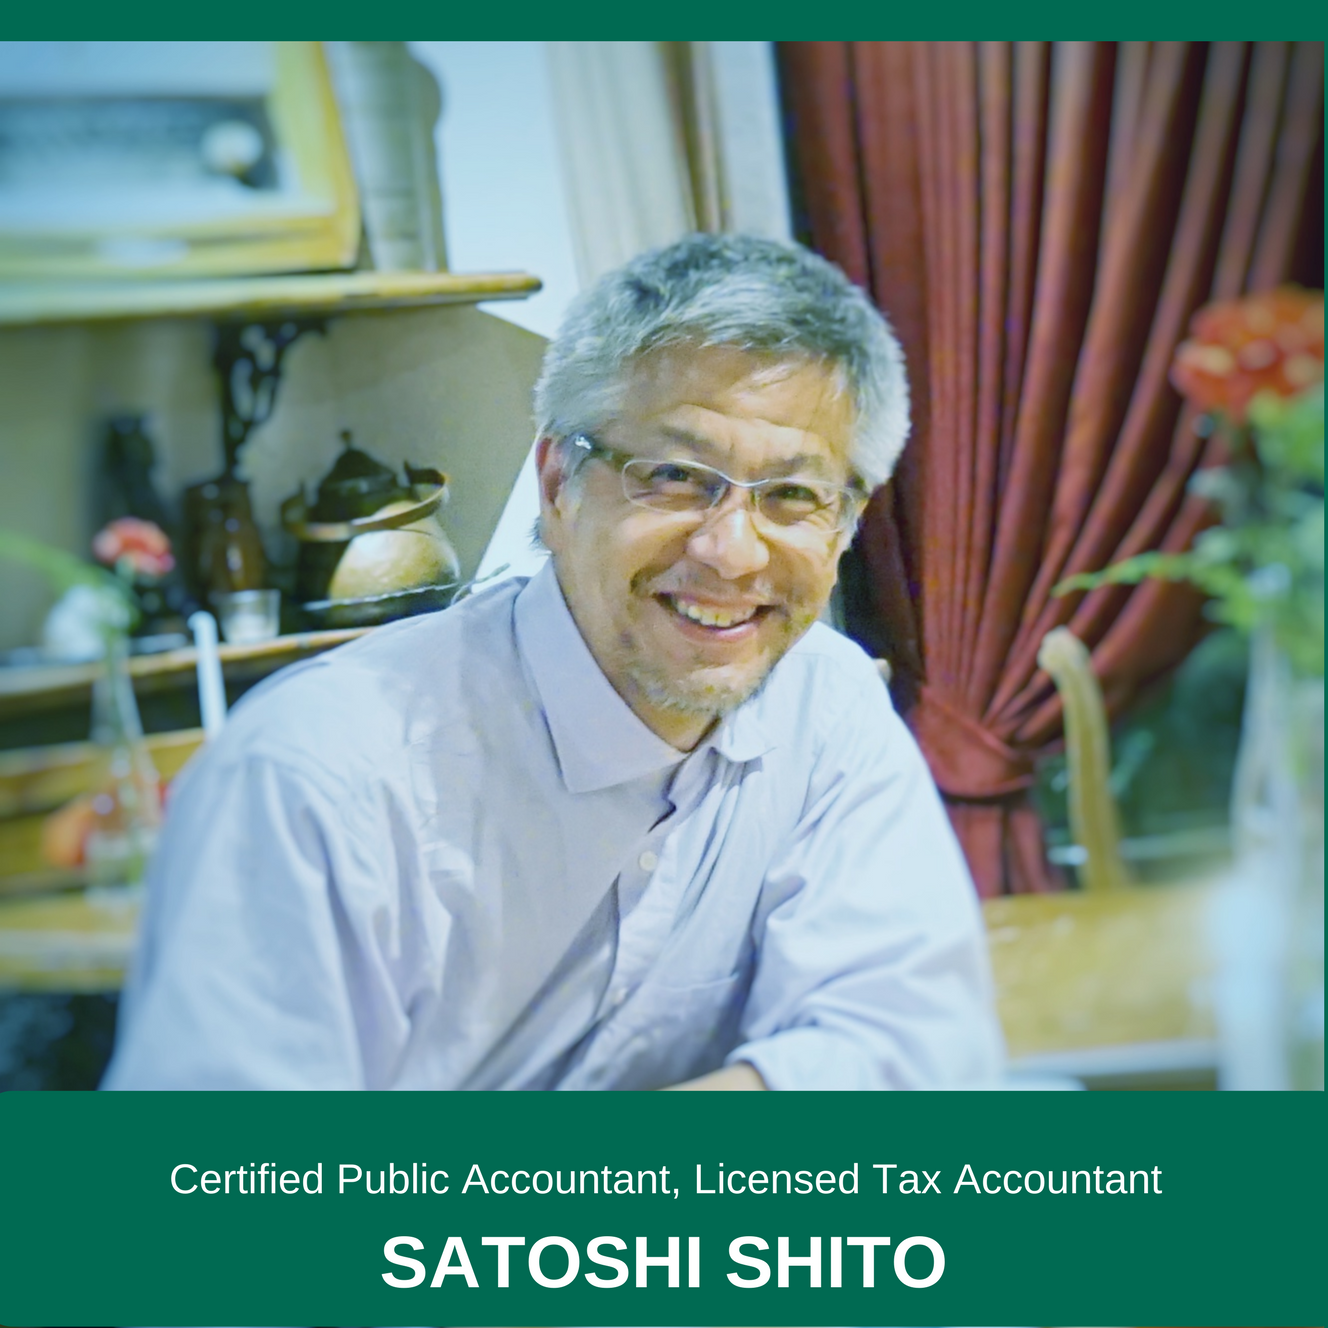
\includegraphics[width=35mm]{shirokanecpa.png}
%\end{wrapfigure}
\end{minipage}

\vspace{-40mm}    %横書き用
\section{My Profile}

\subsection{Personal Information}

\begin{table}[h]
%\begin{spacing}{0.9}
  \begin{tabular}{lll}
Name & {\sffamily \bfseries SATOHSI SHITO} & \\
Professional & \multicolumn{2}{l}{Certified Public Accountant, \textit{1999 (No. 020888)}} \\
\ licenses       & \multicolumn{2}{l}{Certified Tax Accountant, \textit{2013 (No. 127096)}} \\
Affiliation  & \multicolumn{2}{l}{Tokyo Tax Accountant Agency,} \\
 & \multicolumn{2}{l}{Tax Support committee at Shinagawa} \\
         & \multicolumn{2}{l}{Japan CPA Tax committee} \\
         & \multicolumn{2}{l}{Certified Support Agencies for Business Innovation} \\

\includegraphics[width=4mm]{phone.png} & {\sffamily \bfseries +81 80-1257-5877} & \\

\includegraphics[width=4mm]{mail.png} & {\sffamily \bfseries satoshi.shito@shirokanecpafirm.com} & \\

\includegraphics[width=4mm]{website.png} & \multicolumn{2}{l}{\href{https://www.shirokanecpa.com/}{En) https://www.shirokanecpa.com/}} \\
%            & \multicolumn{2}{l}{\href{https://www.shirokanecpafirm.com/}{Jp) https://www.shirokanecpafirm.com/}} \\

\includegraphics[width=4mm]{linkedin.png} & \multicolumn{2}{l}{https://www.linkedin.com/in/satoshishito/} \\    

\includegraphics[width=4mm]{facebook.png} & \multicolumn{2}{l}{Jp)https://www.facebook.com/shirokanecpafirmjp/} \\
            & \multicolumn{2}{l}{En) https://www.facebook.com/Shirokanecpafirm/} \\   
  \end{tabular}
%\end{spacing}
\end{table}

\subsection{Mission}

My objective is to offer adept guidance and steadfast support to entrepreneurs as well as small and medium-sized enterprises. Additionally, I strive to facilitate seamless communication between foreign nationals and the Japanese business community. Rooted in this mission, my commitment lies in nurturing growth and fostering success for all stakeholders as we collectively navigate the path forward into the future.

\subsection{Professional Career Summary}

\subsubsection{M\&A Excellence}

I founded Shirokane CPA Firm on June 25, 2013, in collaboration with esteemed professionals, establishing a boutique consultancy offering specialized financial and tax advisory services. My proficiency spans extensive financial and tax due diligence for Tokyo Stock Exchange-listed entities engaged in M\&A transactions. Moreover, I possess a proven track record in overseeing both statutory and non-statutory audits for discerning clientele.

\subsubsection{Cross-Border Collaboration \& Hong Kong IPO with IFRS}

A significant facet of my journey has centered on nurturing emerging IT venture enterprises, guiding them through intricate tax compliance and strategic business alignment. Leading the audit engagement for Microsoft Japan KK stands as a testament to my leadership. With precision, I directed a dedicated team while concurrently assuming responsibilities as the conduit for Japanese statutory audit, and as a component auditor within Deloitte Seattle's cross-border Microsoft Corp. project. This involvement facilitated seamless collaboration across international boundaries, interfacing with teams in Seattle, Shanghai, and Singapore, fortifying my global perspective on intricate cross-border financial frameworks.

Pioneering noteworthy accomplishments, I orchestrated the groundbreaking Japanese public offering on the Hong Kong Stock Exchange in 2011. Expertly overseeing a Japanese professional team, I meticulously synchronized efforts with the Hong Kong Deloitte team, culminating in the triumphant IPO of SBI Holding, Inc., a prominent force in the Japanese brokerage landscape listed on the Tokyo Stock Exchange.

\subsubsection{Transformation and Strategy in IPO Preparation}

Within Deloitte's Integrated Service Department, I masterminded the metamorphosis of PGM Golf Group in preparation for their Initial Public Offering (IPO). Harnessing my adeptness, I orchestrated strategic transitions and effectively steered the divestiture of credit holdings from Japanese financial institutions. My purview extended to executing post-IPO group audits for a diverse pool of up to 40 companies, and providing strategic counsel on Japan Internal Control Audit intricacies.

My illustrious 19-year CPA career spans partnerships with over 130 diverse companies, evaluating the intricacies of approximately 30 M\&A opportunities. These multifaceted experiences have endowed me with a profound comprehension of varied management paradigms, refining my discernment in critical decision-making, and accentuating the imperative of context-sensitive strategies. From shaping organizational frameworks to orchestrating seamless departmental dynamics and sculpting pragmatic crisis mitigation strategies, I am resolutely prepared to seamlessly integrate my comprehensive expertise and business acumen to surmount future challenges.


%\subsection{Personal Activities}

%{\bfseries \itshape Down-hill Skiing (off-piste):} \\
%From the top of following mountains, \\
%Mt. Fuji (\textit{the highest in Japan, 2012, 2013, and 2014}) \\
%Okuhodaka (\textit{3rd highest in Japan, 2013}) \\
%Harinoki (\textit{2,821m, 2008, 2009}), Tanigawa (\textit{1,977m, 2012-}) \\

%{\bfseries \itshape Traveling:} \\
%California and Oregon, U.S.  (\textit{1991})\\
%Austria (\textit{1998}), Australia (\textit{1998}) \\
%Poland and Estonia (\textit{2015}) \\
%Croatia, Bosnia and Herzegovina, and Montenegro (\textit{2016}) \\
%Domestic area \\
             
%{\bfseries \itshape Scuba Diving:} \\       
%Certification of Advanced Open Water Diver. Experience of \\
%TAKA Dive's 5days cruise  (\textit{1999}) and two 4days diving trips with catamaran yacht at Okinawa, Japan (\textit{2008, 2000}). \\






\end{document}

%=======テンプレ======

\section{}
\subsection{}

\begin{coloritemize}
\begin{spacing}{0.95}
  \item 
  \item 
  \item 
  \item 
%  \item 
\end{spacing}
\end{coloritemize}

%======右側折り返しの表(タイトル4文字のケース)28文字を調整して利用======
\begin{table}[h]
  \begin{tabular}{lcp{28em}}
    氏名 & : & Giovvani Pellone, ジォバニ・ペローネ \\
    住所 & : & 東京都目黒区上目黒3-12-23-308 \\
    生年月日 & : & 1964年7月18日 \\
    国籍 & : & イタリア \\
    VISA & : & 就労制限なし \\
    結婚 & : & 既婚(日本人) \\
    職業 & : & 工業デザイナー、クリエイティブ・ディレクター、グラフィック・デザイナー \\
  \end{tabular}
\end{table}

%======表
\begin{minipage}{120mm}
  \begin{tabular}{llll}
\hline
 事業の種類   & 主な収入 & 会計納税単位 & 備考 \\
\hline
  Airbnb事業 & ホストからの手数料収入 & 一般財団法人 & 地域活性化という公共性強調 \\
  ピザ屋 & 飲食店売上 & 株式会社\footnote{当初はアメリカン・ダイナーと同一法人で事業を開始し、後にアメリカン・ダイナーの会社を設立し、必要資産を営業譲渡する方法も考えられます。} & 初期投資が必要、従業員あり \\
  アメリカン・ダイナー & 飲食店売上 & 株式会社 & 初期投資が必要、従業員あり \\
  ヨガ・スタジオ事業 & レッスン料収入 & 個人事業主 & 河辺家の節税目的 \\
  河辺さん個人 & 一般財団法人からの給与所得 & 個人事業主 & \\
  & 飲食会社からの役員報酬 &  & \\
  \hline
  \end{tabular}
\end{minipage}